\documentclass{article}
\usepackage{graphicx}
\usepackage{amsmath}
\usepackage{amssymb}
\usepackage{listings}
\usepackage{xcolor}
\usepackage{tcolorbox}
\usepackage{caption}
\usepackage[hidelinks]{hyperref}
\setlength{\parindent}{0pt}
\usepackage[margin=0.5in]{geometry}

% For graphing
\usepackage{tikz}
\usepackage{pgfplots}
\pgfplotsset{compat=1.15}
\usepackage{mathrsfs}
\usetikzlibrary{arrows}

\usepackage{pst-plot}

\newcommand{\setExerciseNumber}[1]{%
    \begin{titlepage}
        \vbox{ }
        \vbox{ }
        \begin{center}
            % Set course here
            
\includegraphics[width=0.40\textwidth]{../img/NTNU_logo.png}\\[1cm]
            \textsc{\Large TTK4135 - Optimization and Control}\\[0.5cm]
            \vbox{ }

            % Set title here
            { \huge \bfseries Exercise \##1}\\[0.4cm]

            \large
            \emph{Author:}\\
            Sondre Pedersen
            \vfill

            {\large\today}
        \end{center}
    \end{titlepage}
}

\definecolor{framecolor}{HTML}{94a3b8}
\definecolor{bgcolor}{HTML}{cbd5e1}

\newtcolorbox{problem}[2][]{
  colback=bgcolor,
  colframe=framecolor,
  fonttitle=\bfseries\color{black},
  title=Problem #2,
  width=\textwidth,
  #1
}

% Subtask 
\newcommand{\SUBTASK}[2]{\medskip\medskip\textbf{\large (#1) #2}\medskip}

% Matrix shorthand
\newcommand{\M}[1]{\begin{bmatrix} #1 \end{bmatrix}}

% Subheader for smaller sections
\newcommand{\subheader}[1]{\vspace{1em}\noindent\underline{\textbf{\large #1}}\vspace{0.5em}}


\begin{document}

\setExerciseNumber{1}

%%% QUESTION %%%

\begin{problem}{1: The Rosenbrock function}

Compute the gradient $\nabla f(x)$ and Hessian $\nabla ^2 f(x)$ of the Rosenbrock function
\[
  f(x) = 100(x_2 - x_1^2)^2+ (1-x_1)^2
.\] 

Show that $x^* = (1,1)^{\top}$ is the only local minimizer of this function, and that the Hessian matrix at that point 
is positive definite. 

\end{problem}

%%% SOLUTION %%%

\[
  \nabla f(x) = \M{200(x_2-x_1^2)(-2x_1)-2(1-x_1) \\ 200(x_2-x_2^2)} = \M{-400(x_1x_2-x_1^3) + 2x_1-2 \\ 200(x_2-x_1^2)}
.\] 

\[
  \nabla ^2 f(x) = \M{-400x_2+1200x_1^2+2 & -400x_1 \\ -400x_1 & 200}
.\] 

$\nabla f(x) = 0$ at the points where x is a local minimizer. We have that
\begin{itemize}
  \item $200(x_2-x_1^2) = 0 \implies x_2 = x_1^2$
  \item $-400(x_1x_2-x_1^3) + 2x_2 - 2 = 0 \implies -400(x_1^3 - x_1^3) + 2x_1 - 2 = 0 \implies x_1 = 1 = x_2$
\end{itemize}

So $x_1 = x_2 = 1$ is the only minimizer for this function. 

The Hessian matrix at that point is $\M{802 & -400 \\ -400  & 200}$. 

Since the top left element is positive and the determinant is positive ($802*200-400*400$), the Hessian is positive definite. 


%%% QUESTION %%%

\begin{problem}{2: Model Predictive Control}
  Use the same model as Problem 1
  
  \medskip (a) Provide a short explanation of the MPC principle.
  
  \medskip (b) Assume that full state measurements are available. 
  Solve this with control horizon length N = 30. Compare with earlier results.
  
  \medskip (c) Use a shorter time horizon and comment on differences. 
  
  \medskip (d) Assume that the model from task 1 is imperfect. The A matrix is correct, but B is 
  multiplied with 0.98 (2\% less force from the actuators than expected). 
  
  Run the MPC with the real model as plant model in the control design and modified system in the simulation. Compare
  output $y_t$ and input $u_t$ with the ones obtained earlier.

\end{problem}

%%% SOLUTION %%%

\SUBTASK{a}{MPC principle}

Model predictive control (MPC) is a control strategy where the current control action is determined by solving a finite-horizon open-loop optimal control problem at each sampling instant. The optimization uses the plant's current state as the initial condition and generates an optimal control sequence. Only the first control input from this sequence is applied to the plant, and the process repeats at the next time step.

\SUBTASK{b}{Using full state information}

The controller manages the model/plant mismatch effectively when the force is only 2\%
less than expected. However, further reducing this margin will cause issues. On the other hand, a force that exceeds the expected value is not problematic.

\SUBTASK{c}{Shorter time horizon}

Using a shorter time horizon in MPC typically leads to more reactive but potentially less optimal control. The controller may struggle with long-term planning, leading to more aggressive corrections and potentially higher control effort. Compare the results with 
N=30 to observe how stability, tracking performance, and control smoothness are affected.

\SUBTASK{d}{Imperfection}

introducing model mismatch by scaling 
B down by 2\% will test the controller's robustness. The MPC will be designed assuming the original model, but the simulation will run with the modified dynamics. Compare the output y
A well-tuned MPC should handle small deviations well, but a noticeable performance degradation or steady-state error may appear.
%%% QUESTION %%%

\begin{problem}{3: Search direction}
Consider the function 
\[
  f(x) = (x_1+x_2^2)^2
.\] 
At the point $x_k^{\top} = (1, 0)$ we consider the search direction $p_k^{\top} = (-1, 1)$. Show that $p_k$ is a descent direction, and find all minimizers of 
\[
  \min_{\alpha > 0} f(x_k + \alpha p_k)
.\] 
\end{problem}

%%% SOLUTION %%%

\[
  \nabla f(x) = \M{2(x_1+x_2^2) \\ 4x_2(x_1+x_2^2)}
.\] 

\[
  \nabla f(1, 0) = \M{2 \\ 0}
.\] 

Given $p_k^{\top} = (-1, 1)$, we get that
\[
  \nabla f(1, 0) ^{\top}p_k = \M{2  & 0}\M{-1 \\ 1} = -2
.\] 

Since the result is negative, we have a descent direction. 


\medskip Define $x(\alpha) = x_k + \alpha p_k = \M{1 \\ 0} + \alpha \M{-1 \\ 1} = \M{1 - \alpha \\ \alpha}$. Using this in f(x) gives $f(1-\alpha, \alpha) = ((1- \alpha) + \alpha^2)^2 := g(\alpha)$.
\[
  \frac{dg}{d\alpha} = 2(1-\alpha + \alpha^2) \times (-1+ 2\alpha) = 0 \implies \alpha = \frac{1}{2}
.\] 

%%% QUESTION %%%

\begin{problem}{4: Find optimizers}
Find the \textit{maxima} of the function $f(x) = x_1x_2$ over the unit disc defined by the inequality constraint $x_1^2 + x_2^2 = 1$. Illustrate the gradients of the
active constraint and the objective function at the optimal points.
\end{problem}

%%% SOLUTION %%%

\begin{align*}
  \mathcal{L}(\mathbf{x}, \lambda)        & = x_1x_2 - \lambda_1(x_1^2 + x_2^2-1)                   \\
  \nabla \mathcal{L}(\mathbf{x}, \lambda) & = \M{x_2 -2\lambda x_1                                  \\ x_1 - 2\lambda x_2 \\ -x_1^2 -x_2^2 + 1} = 0 \\
  \implies x_1                            & = x_2 = \pm \frac{1}{\sqrt{2}},\  \lambda = \frac{1}{2}
\end{align*}

\begin{center}
  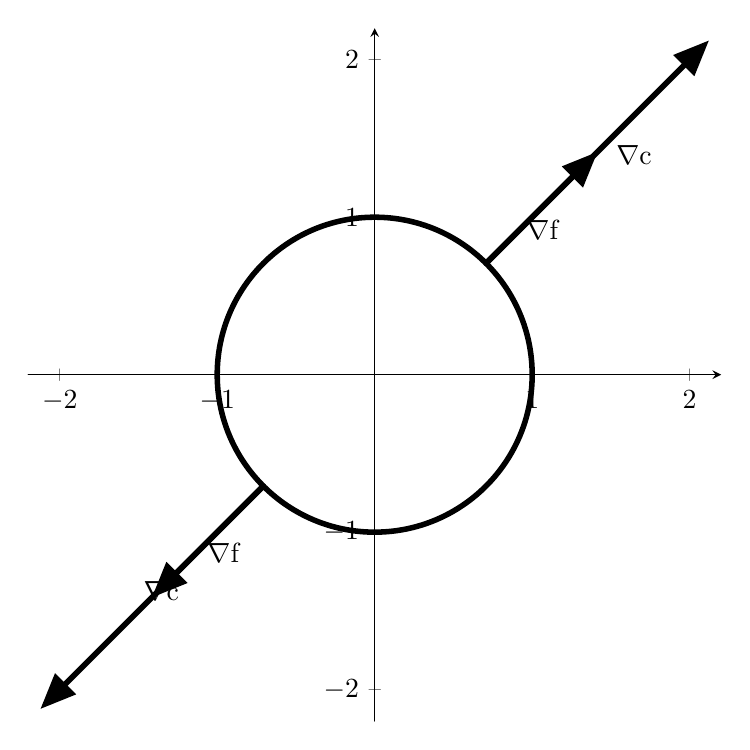
\begin{tikzpicture}[line cap=round,line join=round,>=triangle 45,x=2.0cm,y=2.0cm]
    \begin{axis}[
        x=2.0cm,y=2.0cm,
        axis lines=middle,
        xmin=-2.2,
        xmax=2.2,
        ymin=-2.2,
        ymax=2.2,
        xtick={-2.0,-1.0,...,2.0},
        ytick={-2.0,-1.0,...,2.0},]
      \clip(-2.2,-2.2) rectangle (2.2,2.2);
      \draw [line width=2.pt] (0.,0.) circle (2.cm);
      \draw [->,line width=2.pt] (0.7071067811865475,0.7071067811865475) -- (1.414213562373095,1.414213562373095);
      \draw [->,line width=2.pt] (-0.7071067811865475,-0.7071067811865475) -- (-1.414213562373095,-1.414213562373095);
      \draw [->,line width=2.pt] (0.7071067811865475,0.7071067811865475) -- (2.1213203435596424,2.1213203435596424);
      \draw [->,line width=2.pt] (-0.7071067811865475,-0.7071067811865475) -- (-2.1213203435596424,-2.1213203435596424);
      \begin{scriptsize}
        \draw[color=black] (1.0637954312887226,0.9162861268834652) node {$\nabla$f};
        \draw[color=black] (-0.961618466685309,-1.1309820687316112) node {$\nabla$f};
        \draw[color=black] (1.6466483515690196,1.397139155035049) node {$\nabla$c};
        \draw[color=black] (-1.3550441878745096,-1.3714085828074032) node {$\nabla$c};
      \end{scriptsize}
    \end{axis}
  \end{tikzpicture}
\end{center}

\end{document}
